\documentclass[10pt,letterpaper]{article}
\usepackage[margin=0.75in]{geometry}
\usepackage{amsmath}
\usepackage{amsfonts}
\usepackage{amssymb}
\usepackage{graphicx}
\usepackage{cancel}
\usepackage{listings}
\usepackage{color}
\usepackage{textcomp}
\definecolor{listinggray}{gray}{0.9}
\definecolor{lbcolor}{rgb}{0.9,0.9,0.9}
\lstset{
	backgroundcolor=\color{lbcolor},
	tabsize=4,
	rulecolor=,
% 	language=Python,
        basicstyle=\scriptsize,
        upquote=true,
        aboveskip={1.5\baselineskip},
        columns=fixed,
        showstringspaces=false,
        extendedchars=true,
        breaklines=true,
        prebreak = \raisebox{0ex}[0ex][0ex]{\ensuremath{\hookleftarrow}},
        frame=single,
        showtabs=false,
        showspaces=false,
        showstringspaces=false,
        identifierstyle=\ttfamily,
        keywordstyle=\color[rgb]{0,0,1},
        commentstyle=\color[rgb]{0.133,0.545,0.133},
        stringstyle=\color[rgb]{0.627,0.126,0.941},
}

\def\mbf{\mathbf}
\def\mbb{\mathbb}

\providecommand{\abs}[1]{\left\lvert#1\right\rvert}
\providecommand{\norm}[1]{\left\lVert#1\right\rVert}
\def\d{\mathrm{d}}
\def\e{\mathrm{e}}

\def\y{\mathbf{y}}
\def\f{\mathbf{f}}
\def\g{\mathbf{g}}
\def\b{\mathbf{b}}

\title{Numerical Treatment of Differential Equations: Homework 6}
\author{Truman Ellis}

\begin{document}
\maketitle

Our finite difference code solves Laplace's equation
\[
-\Delta u = f
\]
by approximating the Laplacian with matrix operator $\mbf{A}$. $\mbf{A}$ has
eigenvalues $\lambda^{a,b}=\frac{4}{h^2}\left\{\sin^2\left(\frac{a\pi
h}{2}\right)+\sin^2\left(\frac{b\pi h}{2}\right)\right\}$ and eigenvectors 
$v^{a,b}_{ij}=\sin(ai\pi h)\sin(bj\pi h)$ for $1\le a\,,b\le m$.

If we set $f=\lambda^{a,b}v^{a,b}$ we will be solving the eigenvalue problem
\[
\mbf{A}u=\lambda^{a,b}v^{a,b}
\]
and we should exactly recover the solution $u=v^{a,b}$. Indeed, for various
values of $a$ and $b$ we recover the exact eigenvectors to machine precision as
shown in Figures (1) - (6).

If we instead replace our forcing function with the eigenvalues and eigenvectors
of the continuous operator, $\lambda_{a,b}=(a^2+b^2)\pi^2$ and $v_{a,b}=\sin(a\pi
x)\sin(b\pi y)$, respectively, we can observe the
convergence of our discrete operator to the continuous. The final set of figures
demonstrate this convergence for various values of $a$ and $b$.

\begin{figure}[p]
\begin{center}
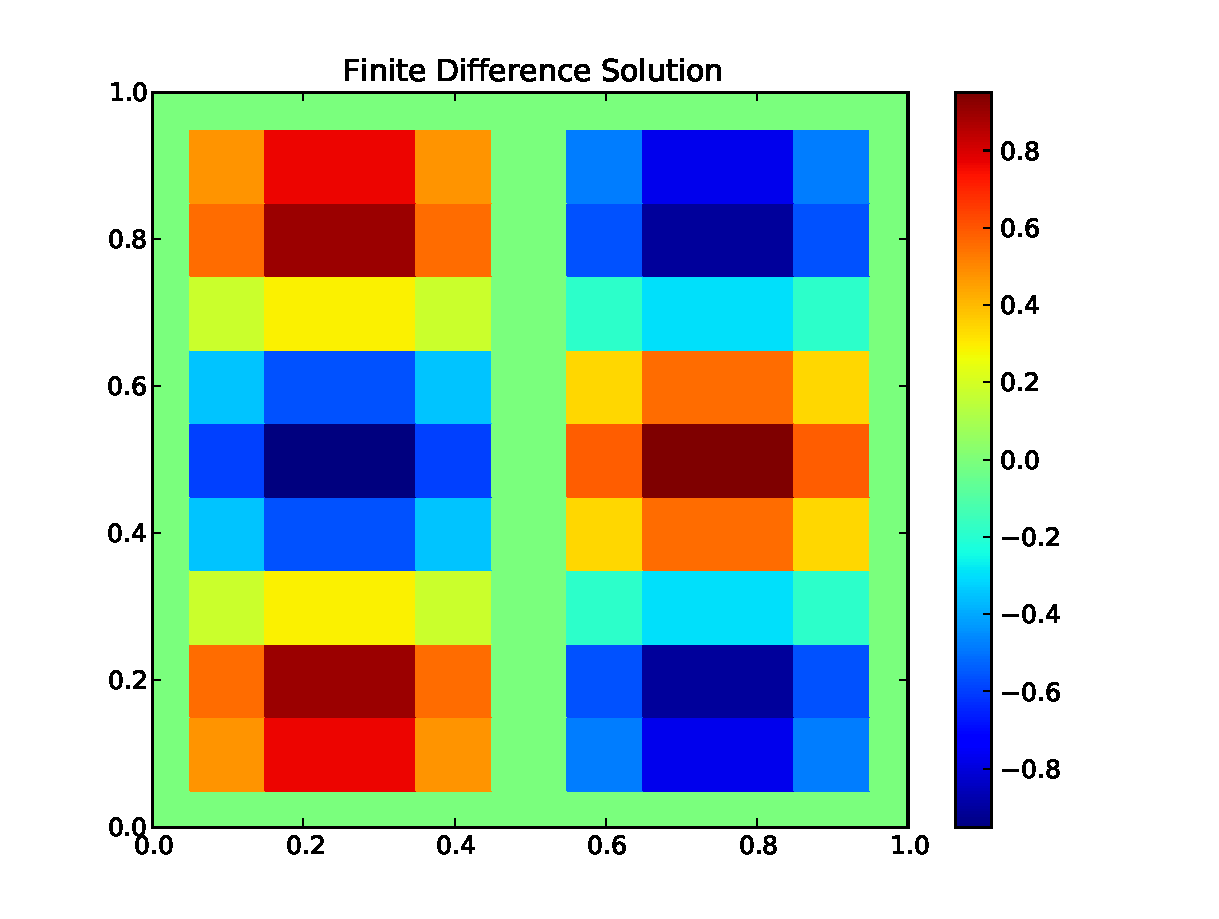
\includegraphics[width=5in,keepaspectratio]{a23.pdf}
\end{center}
\caption{$a=2$, $b=3$, error = $2.24662632e-16$}
\end{figure}

\begin{figure}[p]
\begin{center}
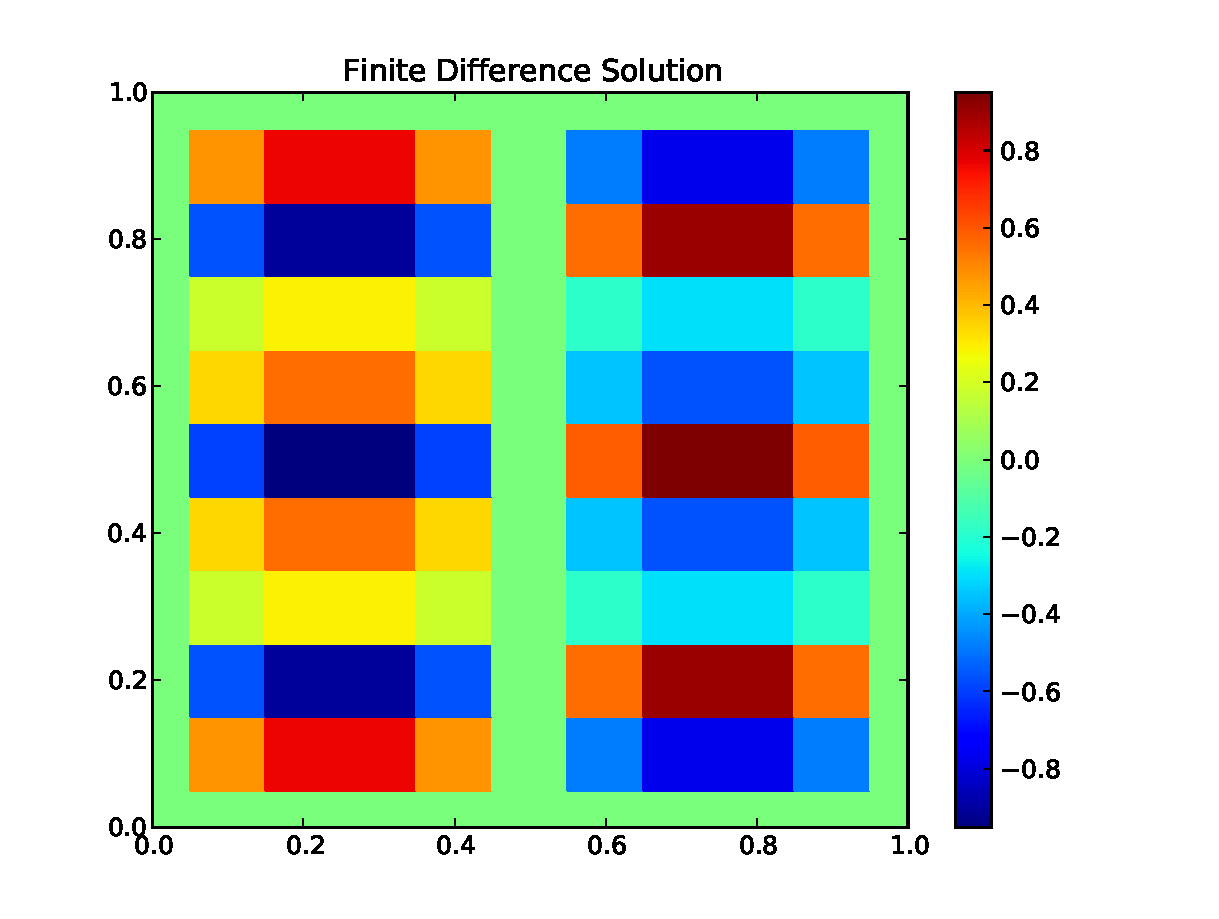
\includegraphics[width=5in,keepaspectratio]{a27.pdf}
\end{center}
\caption{$a=2$, $b=7$, error = $6.56173233e-16$}
\end{figure}

\begin{figure}[p]
\begin{center}
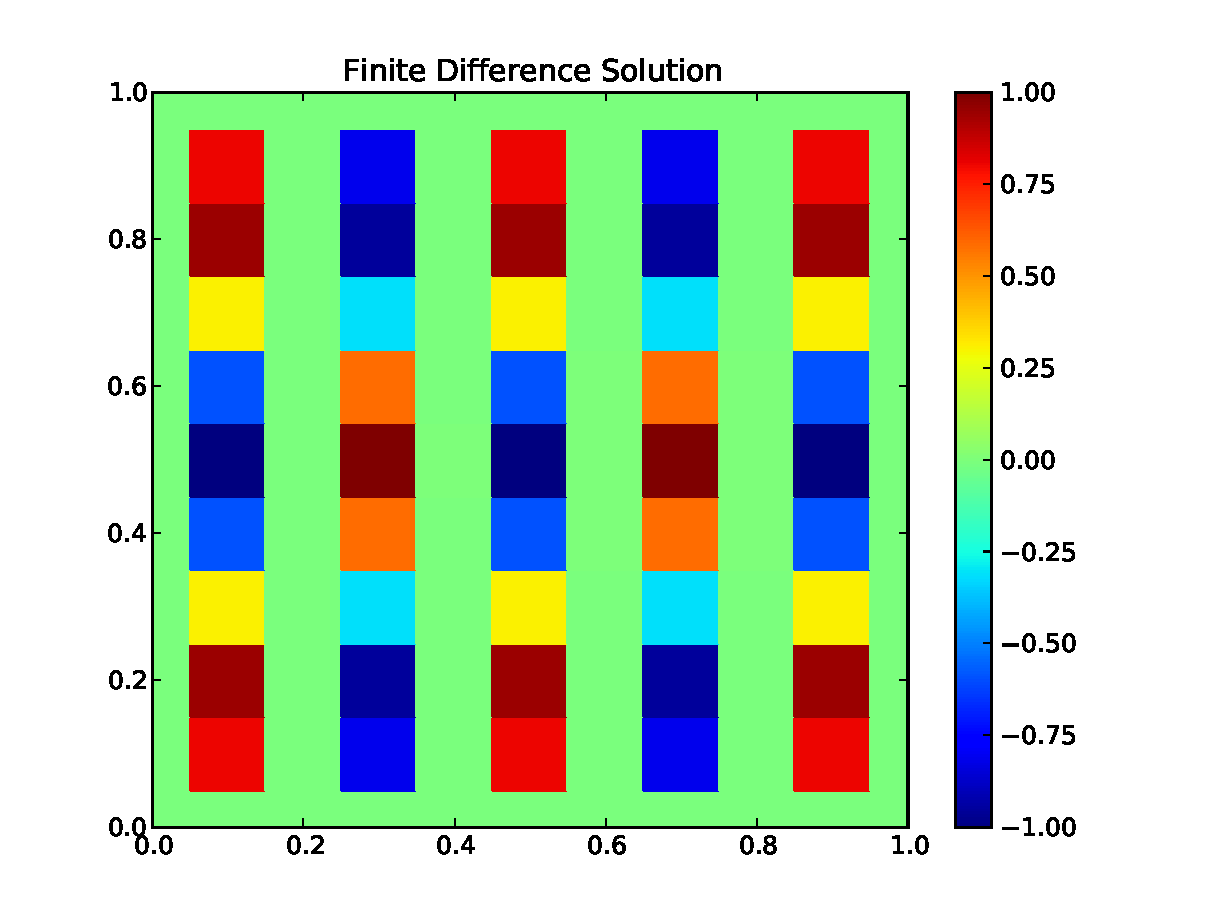
\includegraphics[width=5in,keepaspectratio]{a53.pdf}
\end{center}
\caption{$a=5$, $b=3$, error = $5.12525209e-16$}
\end{figure}

\begin{figure}[p]
\begin{center}
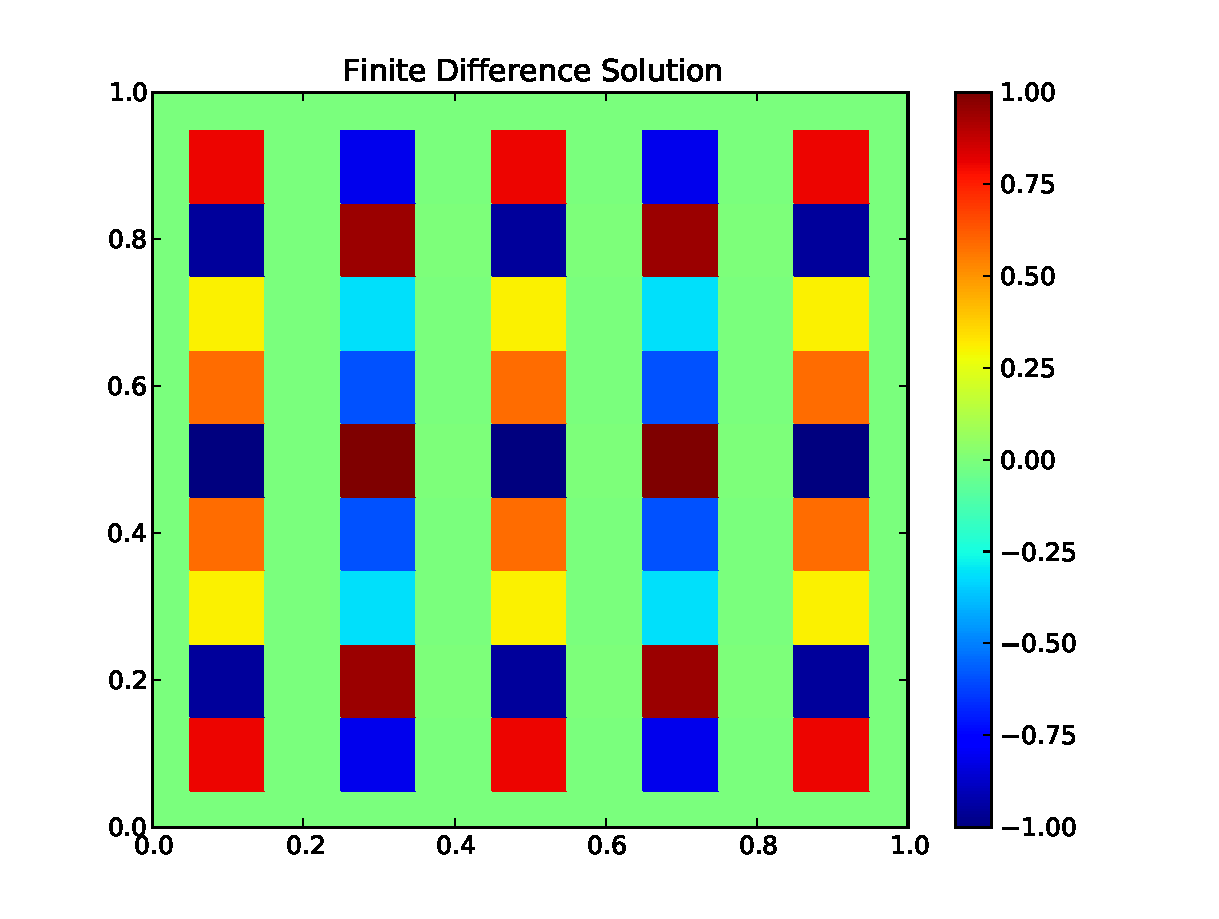
\includegraphics[width=5in,keepaspectratio]{a57.pdf}
\end{center}
\caption{$a=5$, $b=7$, error = $4.37301726e-16$}
\end{figure}

\begin{figure}[p]
\begin{center}
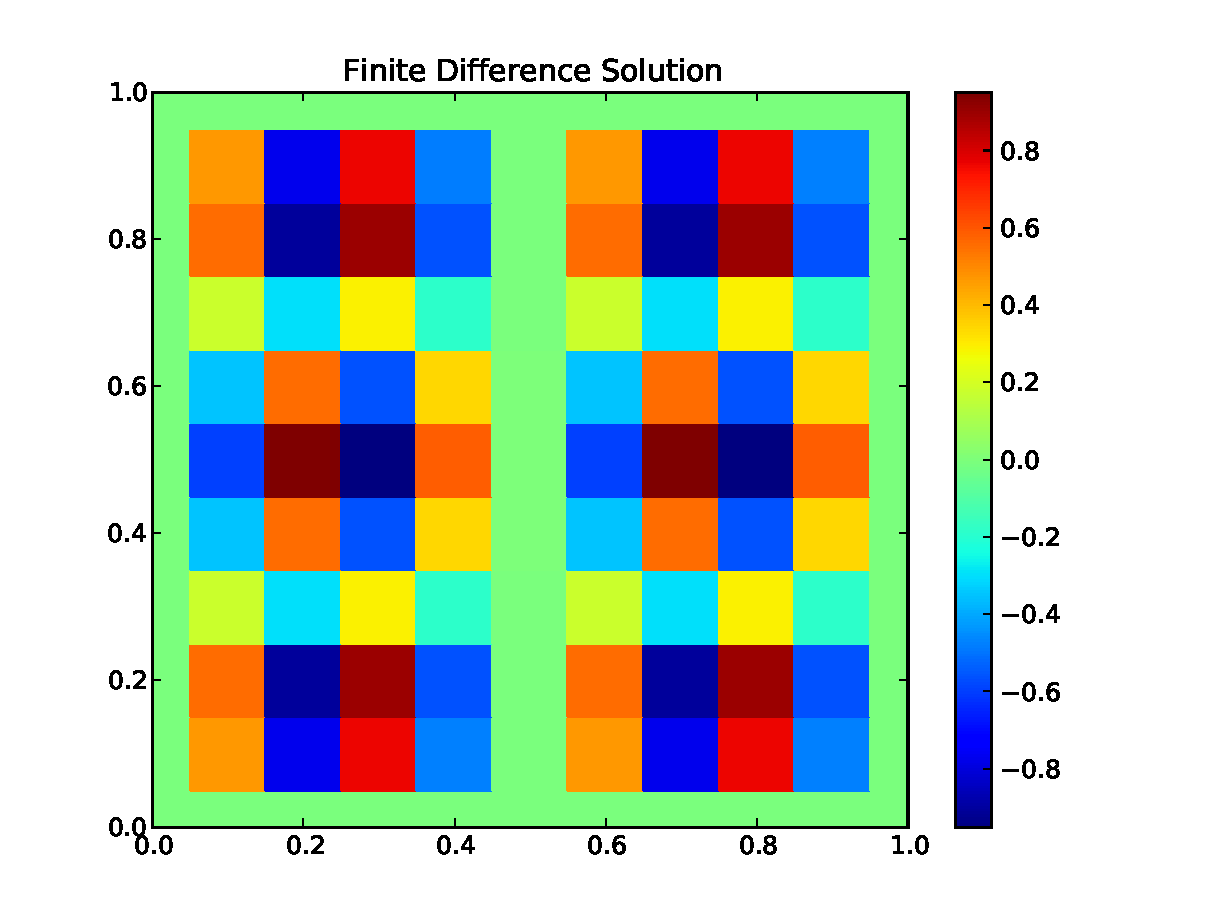
\includegraphics[width=5in,keepaspectratio]{a83.pdf}
\end{center}
\caption{$a=8$, $b=3$, error = $6.98042995e-16$}
\end{figure}

\begin{figure}[p]
\begin{center}
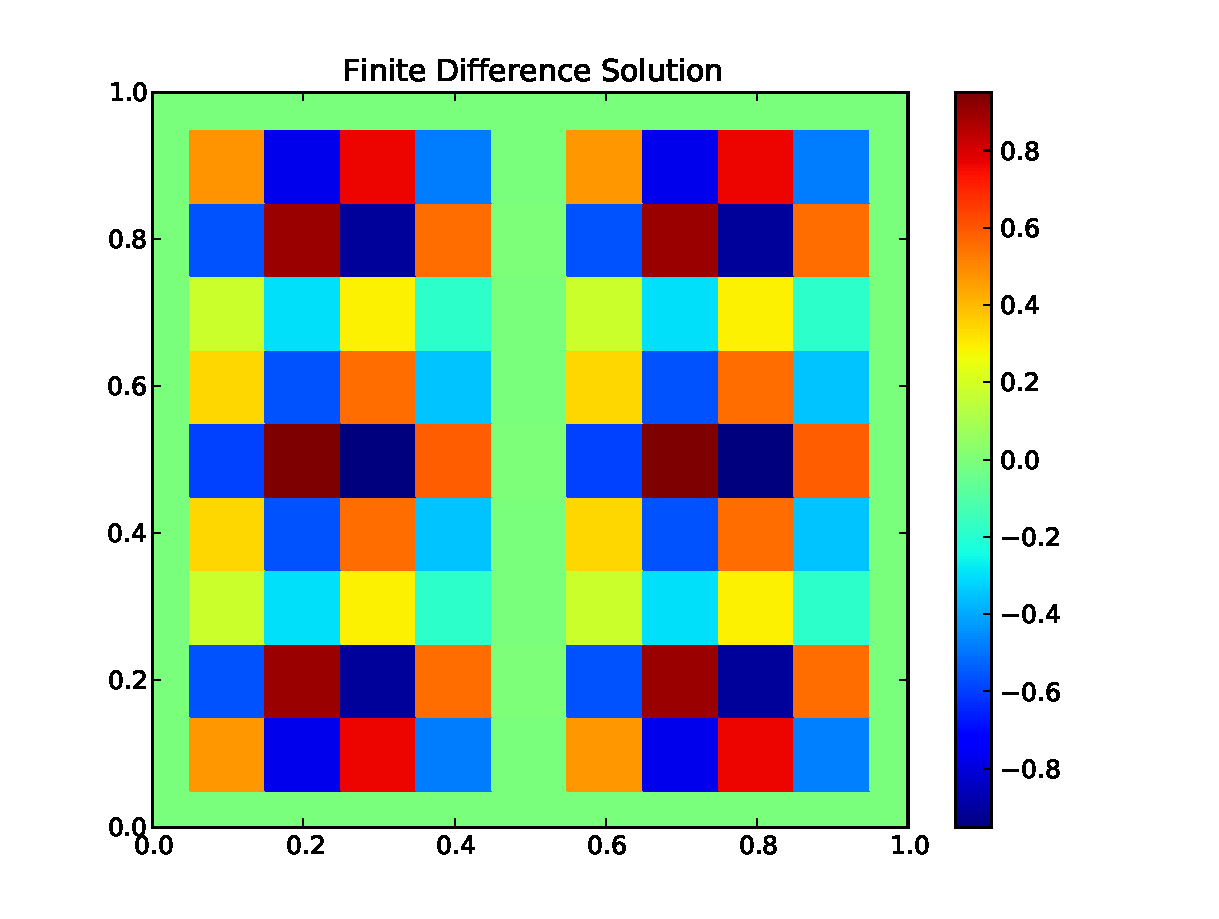
\includegraphics[width=5in,keepaspectratio]{a87.pdf}
\end{center}
\caption{$a=8$, $b=7$, error = $3.56630134e-16$}
\end{figure}

\begin{figure}[p]
\begin{center}
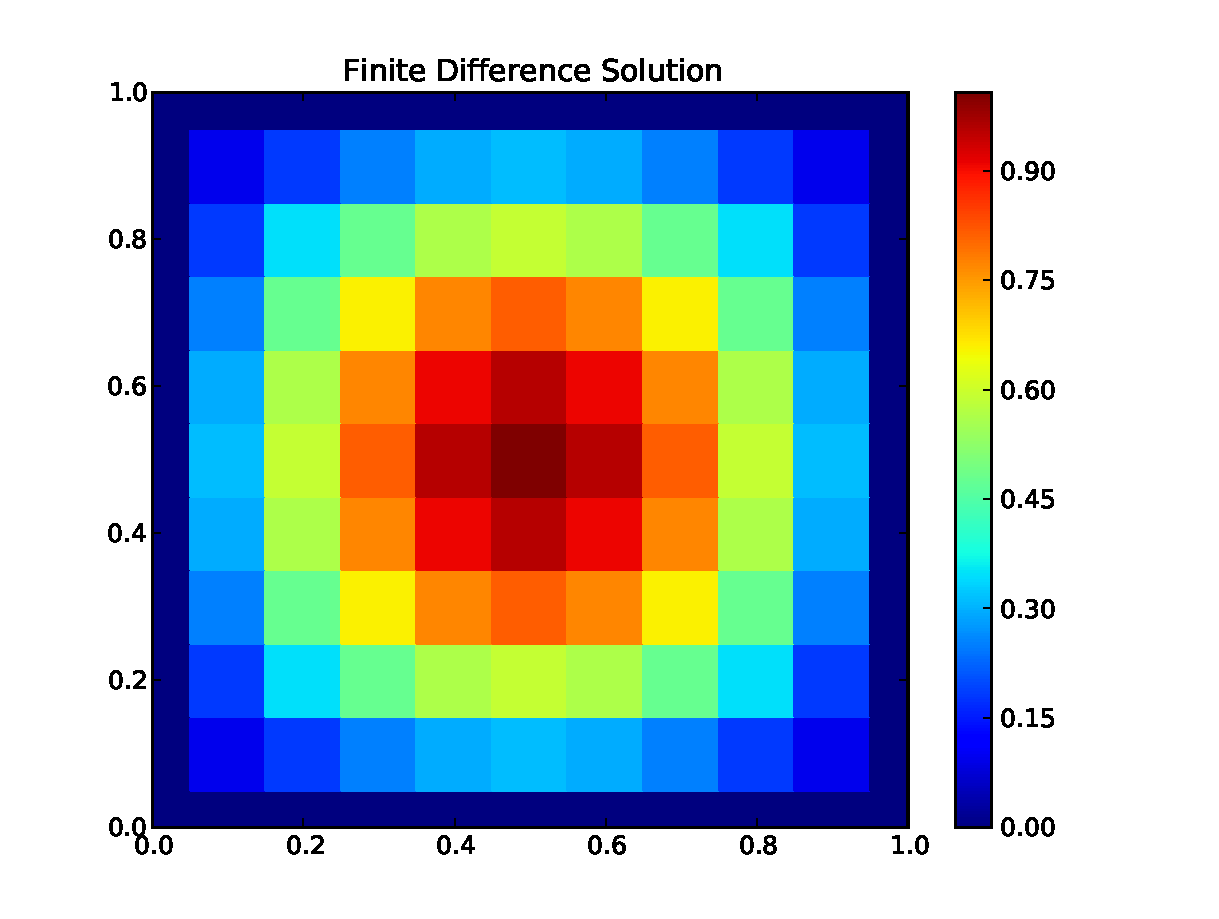
\includegraphics[width=5in,keepaspectratio]{b11.pdf}
\end{center}
\caption{$a=1$, $b=1$: Eigenvector}
\end{figure}

\begin{figure}[p]
\begin{center}
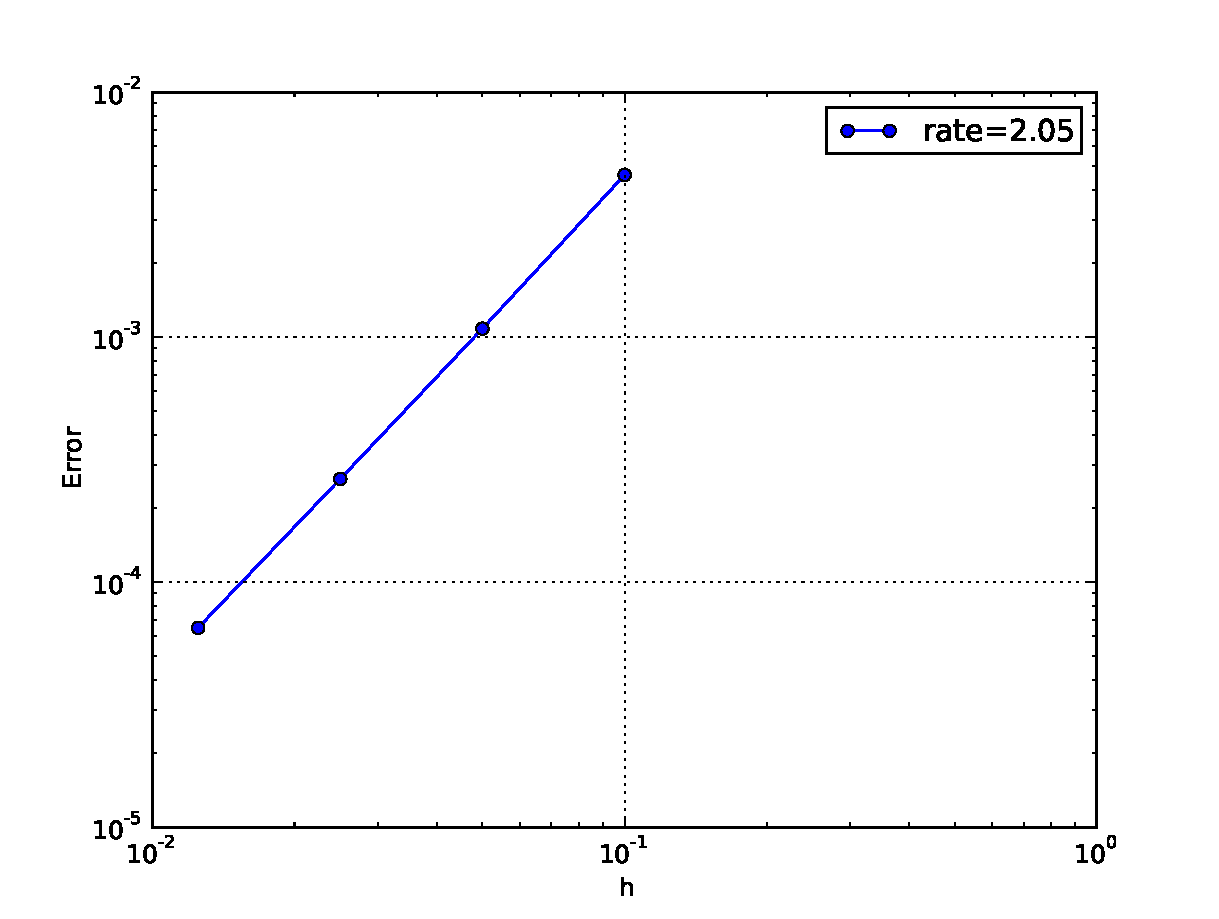
\includegraphics[width=5in,keepaspectratio]{be11.pdf}
\end{center}
\caption{$a=1$, $b=1$: Convergence}
\end{figure}

\begin{figure}[p]
\begin{center}
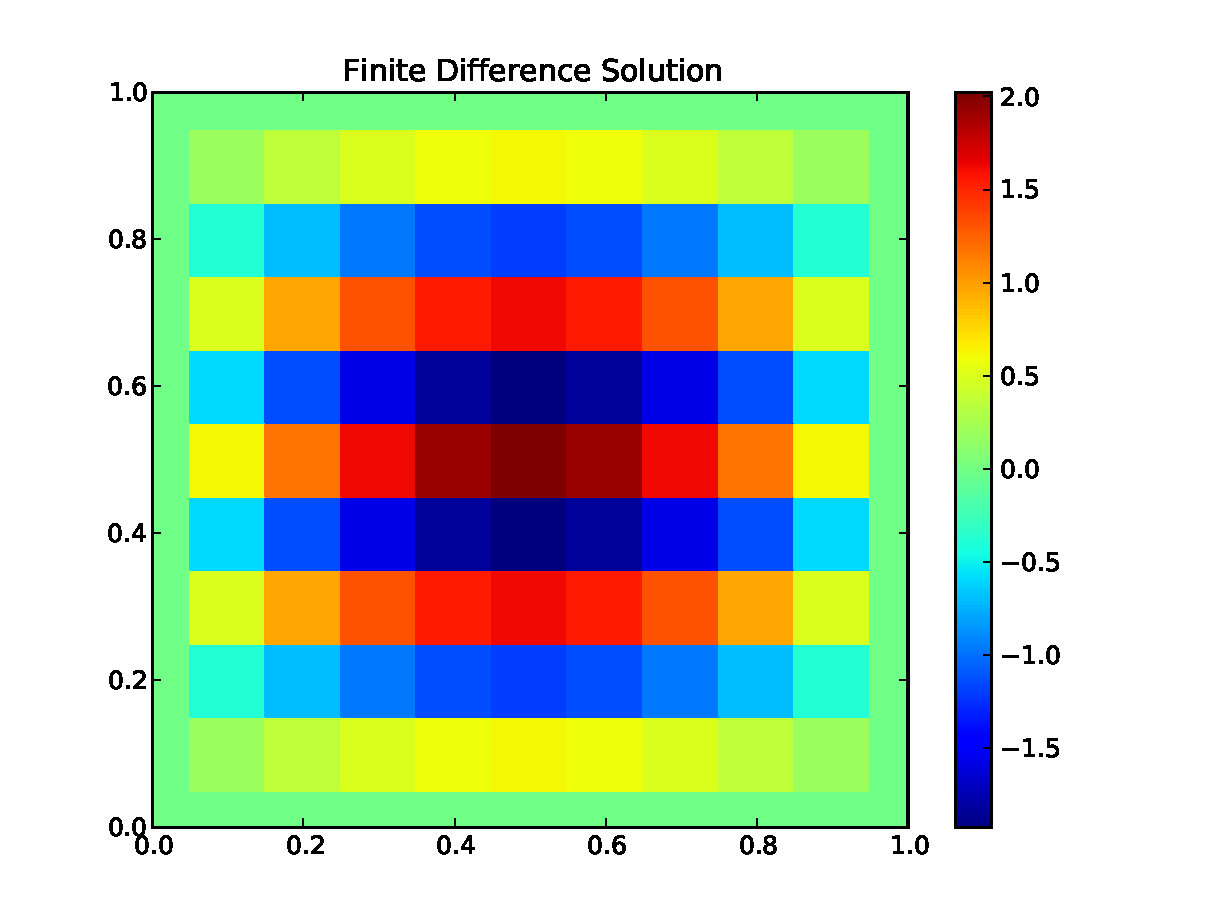
\includegraphics[width=5in,keepaspectratio]{b19.pdf}
\end{center}
\caption{$a=1$, $b=9$: Eigenvector}
\end{figure}

\begin{figure}[p]
\begin{center}
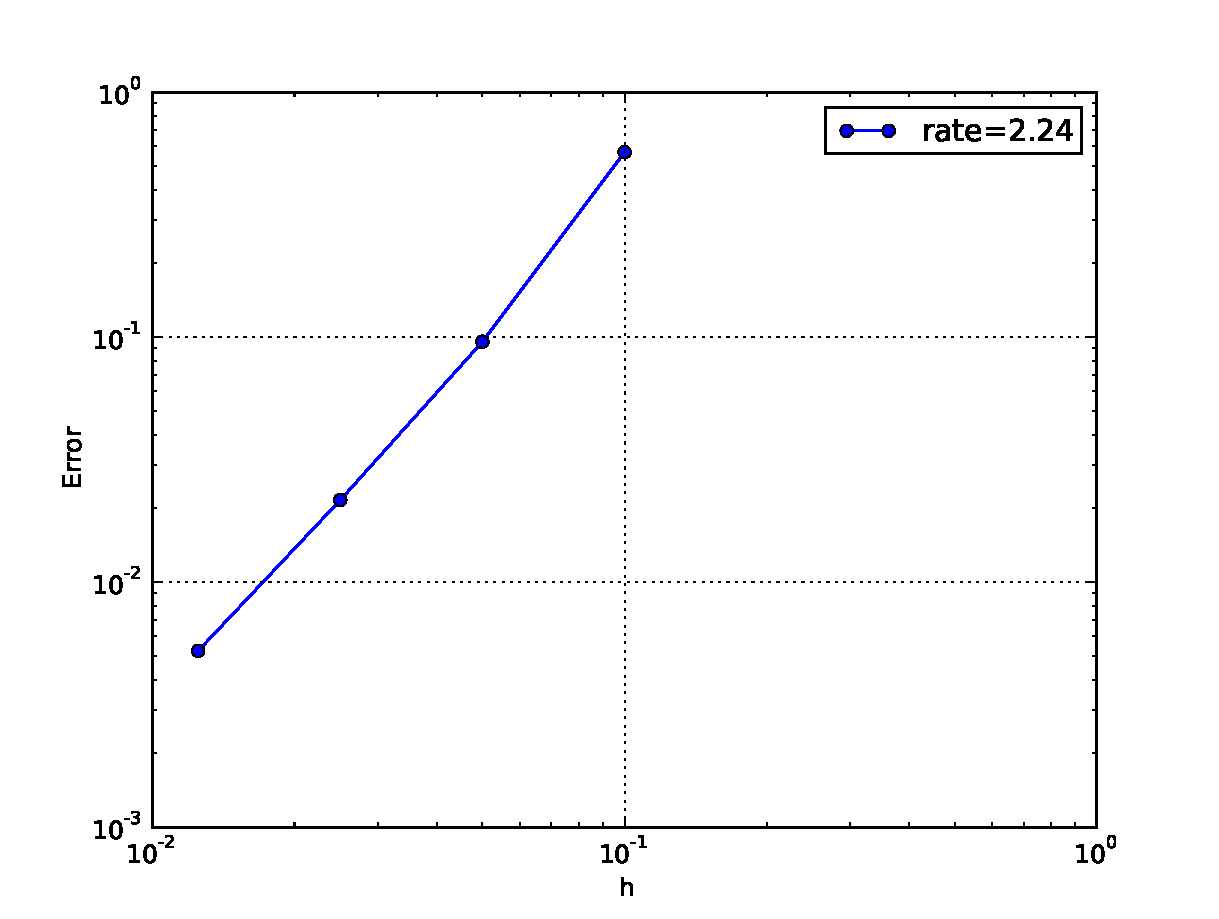
\includegraphics[width=5in,keepaspectratio]{be19.pdf}
\end{center}
\caption{$a=1$, $b=9$: Convergence}
\end{figure}

\begin{figure}[p]
\begin{center}
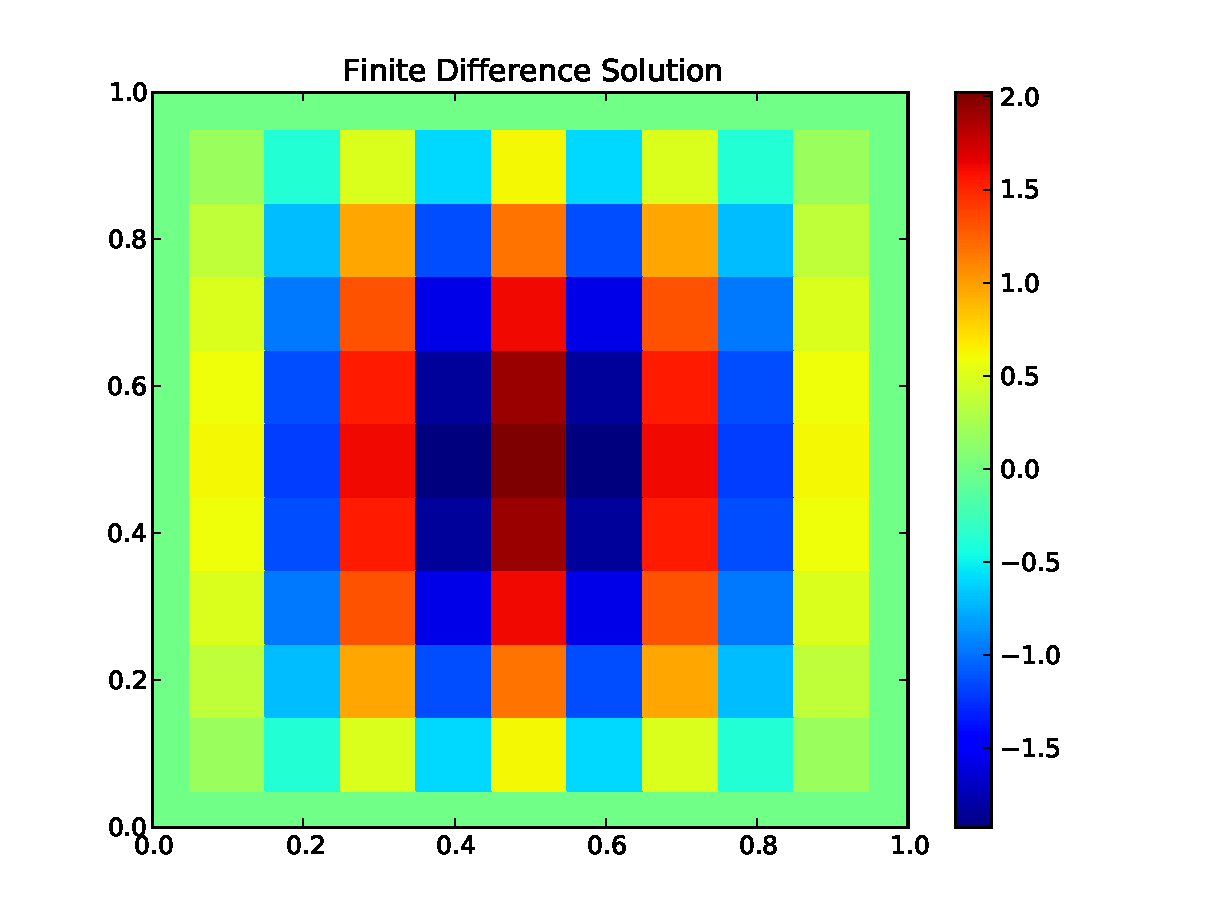
\includegraphics[width=5in,keepaspectratio]{b91.pdf}
\end{center}
\caption{$a=9$, $b=1$: Eigenvector}
\end{figure}

\begin{figure}[p]
\begin{center}
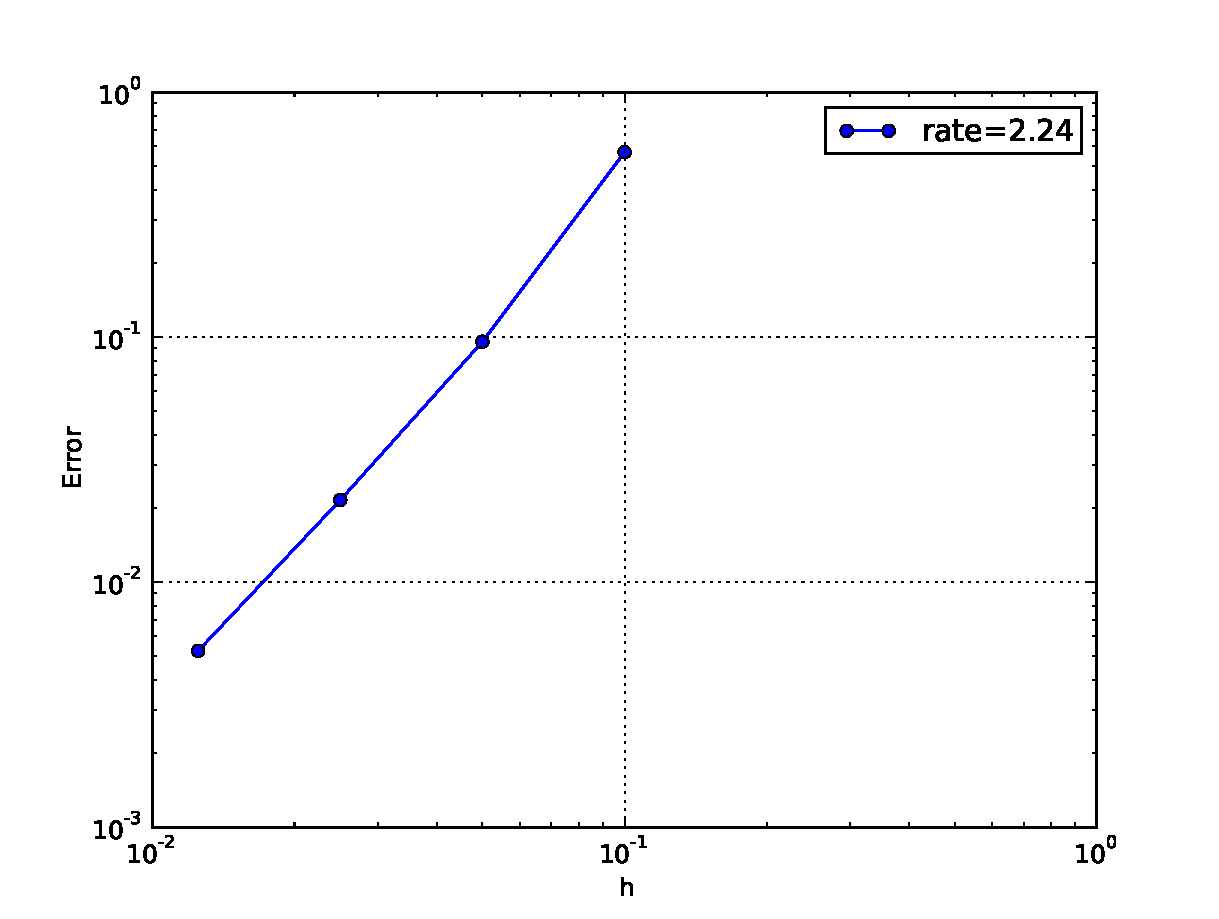
\includegraphics[width=5in,keepaspectratio]{be91.pdf}
\end{center}
\caption{$a=9$, $b=1$: Convergence}
\end{figure}

\begin{figure}[p]
\begin{center}
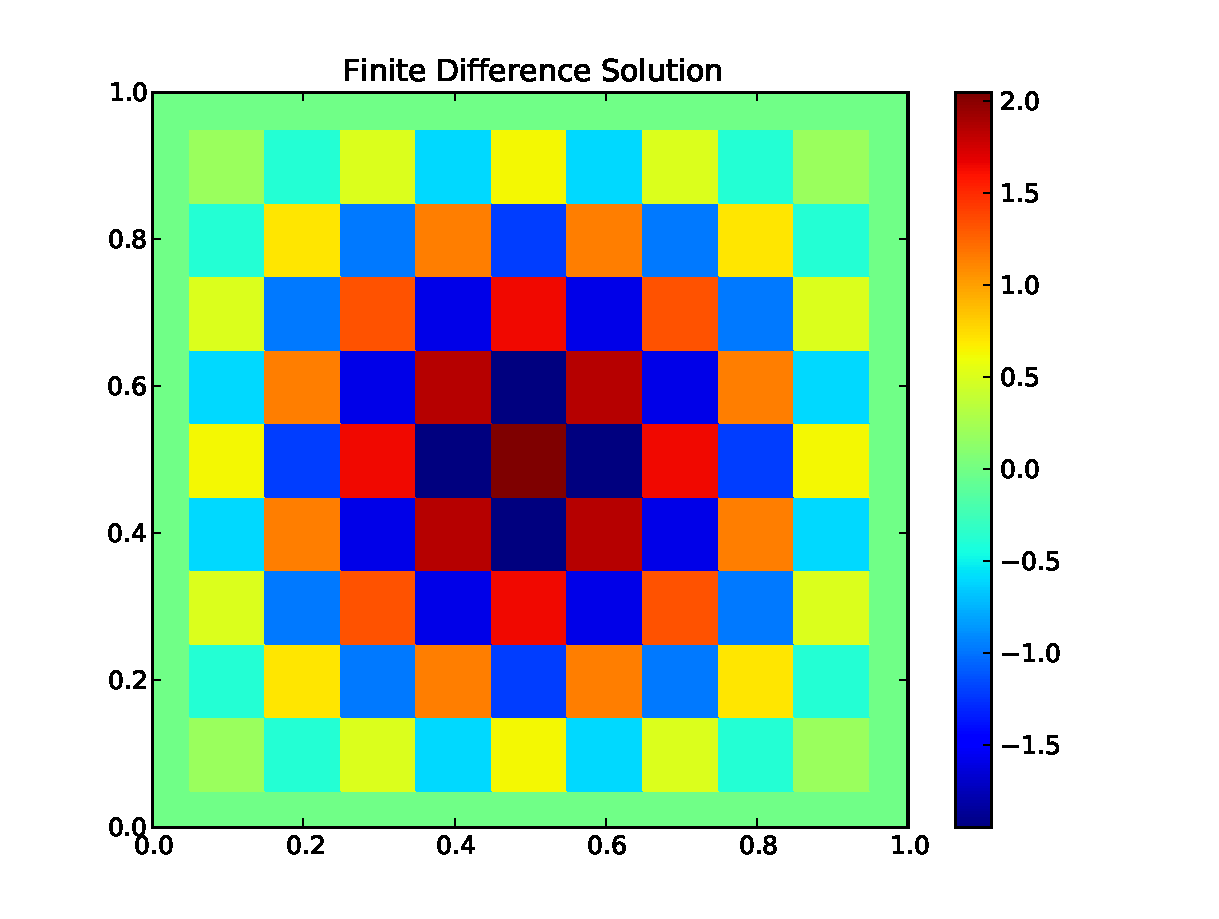
\includegraphics[width=5in,keepaspectratio]{b99.pdf}
\end{center}
\caption{$a=9$, $b=9$: Eigenvector}
\end{figure}

\begin{figure}[p]
\begin{center}
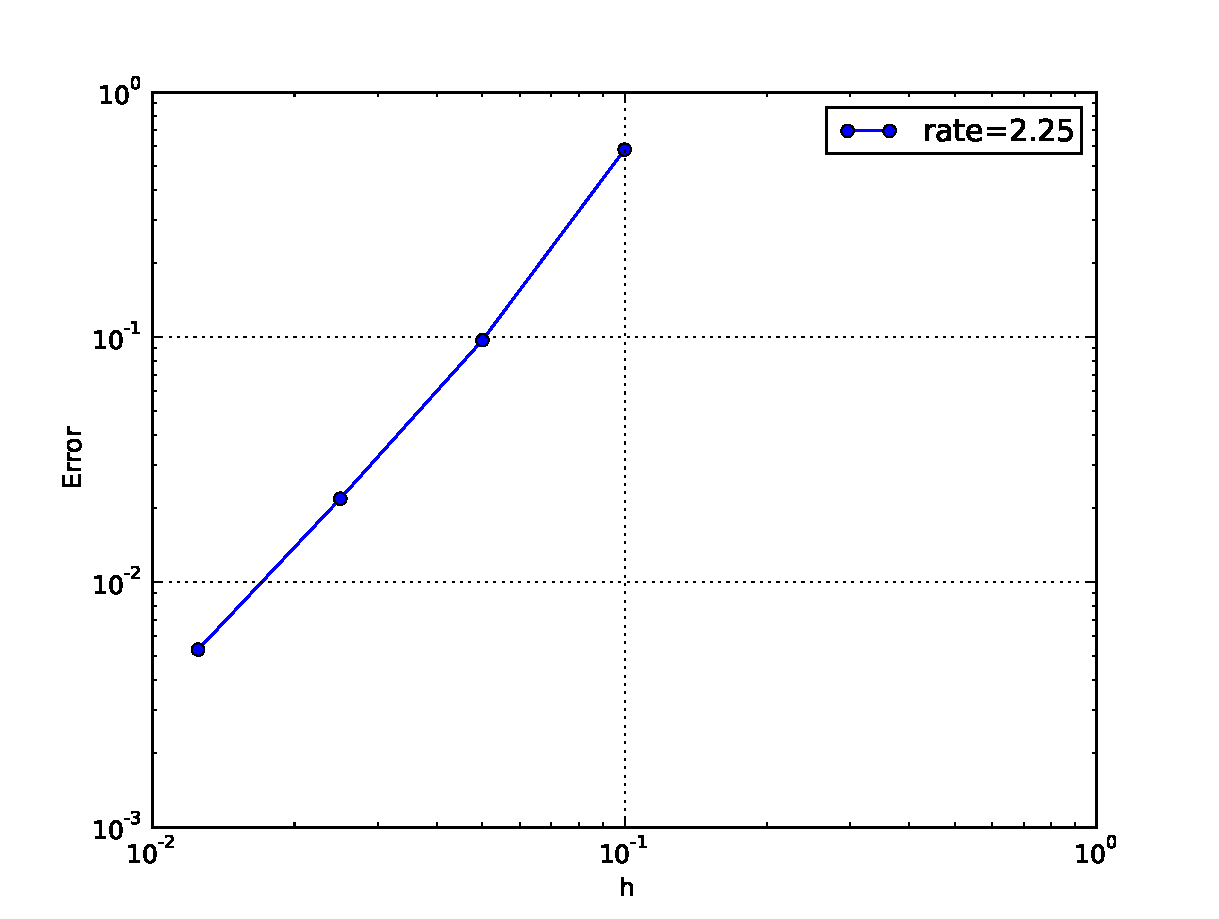
\includegraphics[width=5in,keepaspectratio]{be99.pdf}
\end{center}
\caption{$a=9$, $b=9$: Convergence}
\end{figure}

\clearpage
\newpage
\lstinputlisting[language=Python,title={FDSolver.py}]{FDSolver.py}

\end{document}
